\chapter{Introducción}

Los servicios que utilizamos al navegar por internet, al consultar páginas web o al utilizar \textit{apps} en el móvil, realmente están alojados en un conjunto de ordenadores (denominados \textbf{servidores}) que están almacenados en un \textbf{CPD} (centro de procesamiento de datos).

Hace unos años había empresas pequeñas que contaban con sus propios servidores en sus oficinas, abaratando parte del coste del mantenimiento de los servidores, ya que no tenían que alquilar el espacio o el propio servidor. Si se quedaba pequeño, compraban uno nuevo, o reajustaban los recursos.

Con el avance de internet, han ido surgiendo distintos proveedores que ofrecen servicios para que las empresas puedan contratarlos en condiciones más favorables y en CPDs profesionales. Veremos diferentes tipos de computación y diferenciaremos distintos tipos de “computación en la nube”.



\chapter{Sistemas de computación propios}
Dado que tener el servidor en una oficina puede suponer distintos riesgos (pérdida de electricidad, robo de datos, acceso al servidor por parte de personas no autorizadas, tener la necesidad de tener IP estática en la oficina,...), muchas empresas deciden delegar la parte pública de sus servicios en empresas que cumplen con estándares de seguridad para tener servidores de manera segura.

\infobox{Se siguen teniendo servidores en las oficinas, pero son para tareas internas, de desarrollo o para el control de dominios. \textbf{No es habitual tener servicios externos}.}

Para los servicios externos, dependiendo del tamaño de la empresa, hoy en día lo habitual es delegar parte del mantenimiento o de los servicios en un proveedor externo.

Algunos ejemplos de sistemas de computación propios (cuando nos referimos a \textit{hardware} propio) puede ser:

\begin{itemize}
    \item \textbf{CPD propio}: Esto sólo está al alcance de empresas muy grandes, que necesitan de muchos servidores y que tienen la necesidad de montar su propio CPD parar sus propios servicios.

    \item \textbf{Alquiler de un \textit{rack} en un CPD profesional}: Existen empresas que se encargan de crear CPDs donde alquilan armarios donde poder colocar nuestros servidores físicos. La empresa nos proporcionará el espacio, el ancho de banda que contratemos, y puede que otros servicios extra de red (\textit{firewall} perimetral, sistemas para apaciguar ataques de denegación de servicios...). Por otro lado, el \textit{hardware} del servidor lo proporcionaremos nosotros, y cualquier posible rotura del mismo será cosa nuestra.

    En este tipo de sitios se necesita pedir cita previa para acceder a los servidores, y sólo ciertas personas pre-autorizadas previamente podrán entrar. 

    \item \textbf{Alquiler de máquinas virtuales}: Con el \textbf{\textit{boom}} de la virtualización, surgieron compañías que ofrecen la posibilidad de contratar unos recursos (con computación, RAM y almacenamiento limitados) que están virtualizados dentro de la infraestructura del proveedor. Esto hace que sea barato de contratar, pero toda la gestión del sistema operativo y del software sea por nuestra cuenta.
\end{itemize}


Dependiendo de las necesidades de la empresa, se hará uso de un sistema u otro. El problema en estos casos, es que normalmente es necesario un equipo de informáticos que tengan los conocimientos adecuados dependiendo del tipo de infraestructura que tengamos.

Aunque hoy en día este tipo de computación sigue siendo barato y funcional, el término “computación en la nube” ha hecho que este tipo de contrataciones hayan quedado en parte relegadas.



\chapter{Computación en la nube}

La computación en la nube se puede resumir como el uso de una red de servidores al que de manera remota se puede solicitar una serie de recursos que nos proporcionará de manera casi instantánea, y sin la gestión activa por nuestra parte. Normalmente \textbf{la gestión de todo se puede realizar a través de un panel web de configuración}.

En lugar de solicitar un recurso físico como tal, “la nube”, que está compuesta por un conjunto de servidores que ha sido configurada como “un todo”, es capaz de proporcionarnos distintos tipos de recursos dependiendo de las necesidades que tengamos en ese momento.

Por poner sólo unos ejemplos:

\begin{itemize}
    \item \textbf{Software as a Service} (SaaS): En este caso se contrata lo necesario para poder hacer uso de un software y todo los datos que se vayan a almacenar con él. El proveedor nos da acceso a una instancia del software que está configurada y que permitirá el uso con unos recursos limitados. 
    
    De esta manera, no nos tendremos que preocupar del \textit{hardware} en el que está instalado, o la propia instalación del software. \textbf{Ejemplos}: servicio blog; sistema ERP para una empresa; sistema de base de datos con alta disponibilidad y \textit{backups} incluidos... 

    \item \textbf{Platform as a service} (PaaS): Se nos proporcionará una plataforma donde podremos desplegar o correr el servicio que configuremos por nuestra cuenta. El ejemplo más habitual es el de obtener una máquina virtual donde podremos desplegar el servicio que nos interese instalar.
    
    La ventaja del PaaS es que no nos tenemos que preocupar en qué \textit{hardware} está corriendo, y que en caso de necesidad, podríamos ampliar los recursos de manera sencilla. Como desventaja, es que el coste puede volverse muy elevado y en algunos casos complejo de calcular.
    
    \item \textbf{Infraestructure as a Service} (IaaS): Cuando nos referimos a “Infraestructura” hace referencia a un conjunto de servicios como son la red, el almacenamiento, servidores, virtualización, servicios... El proveedor nos proporcionará un conjunto de servicios que es equiparable a tener una red propia con nuestros propios servidores y servicios.
    
    A la hora de mantener y desplegar este tipo de arquitectura, debemos tener los conocimientos adecuados para saber qué se está realizando. Los proveedores facilitan la labor de realizar los despliegues, pero es tarea de quien realiza la acción de conocer exactamente qué se está haciendo y el coste que tendrá.
\end{itemize}


\chapter{Tipos de computación en la nube}

A la hora de hablar de computación en la nube debemos de distinguir principalmente entre dos tipos. Dependiendo del tamaño de nuestra empresa, del departamento de informática que tengamos, de los conocimientos que tengamos y/o del tiempo que tengamos para aprender, deberemos optar por una o por otra.

\section{Nube privada}

La gestión de una nube privada es aquella que está diseñada para una sola organización, y que será administrada por la propia empresa o con ayuda de terceros. Crear una infraestructura propia para la gestión de una nube privada no es una tarea sencilla, ya que va a requerir de una inversión inicial de dinero para la compra de bastante \textit{hardware}, conocimiento para administrarlo, mantenimiento, posibles cambios a futuro...

\errorbox{\textbf{Crear y mantener una nube privada no es una tarea al alcance de cualquier empresa. Es una labor compleja y cara.}}

Para poder crear una nube privada existe distinta tecnología de orquestación de servicios que se puede utilizar:

\begin{itemize}
	\item \href{https://www.openstack.org/}{Openstack}: Nos permite realizar una infraestructura de nube completa, diferenciando entre nodos de computación, de almacenamiento, ...
	
	\item \href{https://cloudstack.apache.org/}{Apache CloudStack}: permite la gestión de grandes redes de máquinas virtuales para la gestión en alta disponibilidad y alta escabilidad.
	
	\item \href{https://www.proxmox.com/en/proxmox-virtual-environment/overview}{Proxmox}: Proxmox no es un sistema de nube privada como tal, ya que es un sistema de virtualización. Por otro lado, es un sistema que permite crear clústers de nodos de virtualización de manera sencilla, por lo que puede ser utilizado como un primer punto de partida para el inicio de una nube privada.
\end{itemize}


\section{Nube pública}

Un proveedor de nube pública es aquel que ofrece los servicios de su propia infraestructura para la gestión y creación de una infraestructura propia a un cliente a través de una suscripción de pago o a través de un sistema de “pago por servicio”.

Hoy en día los proveedores de nube pública son grandes compañías que ofrecen decenas de servicios que son fácilmente contratables a través de un interfaz de administración web, o también a través de sistemas API para poder automatizar tareas.

\begin{center}
	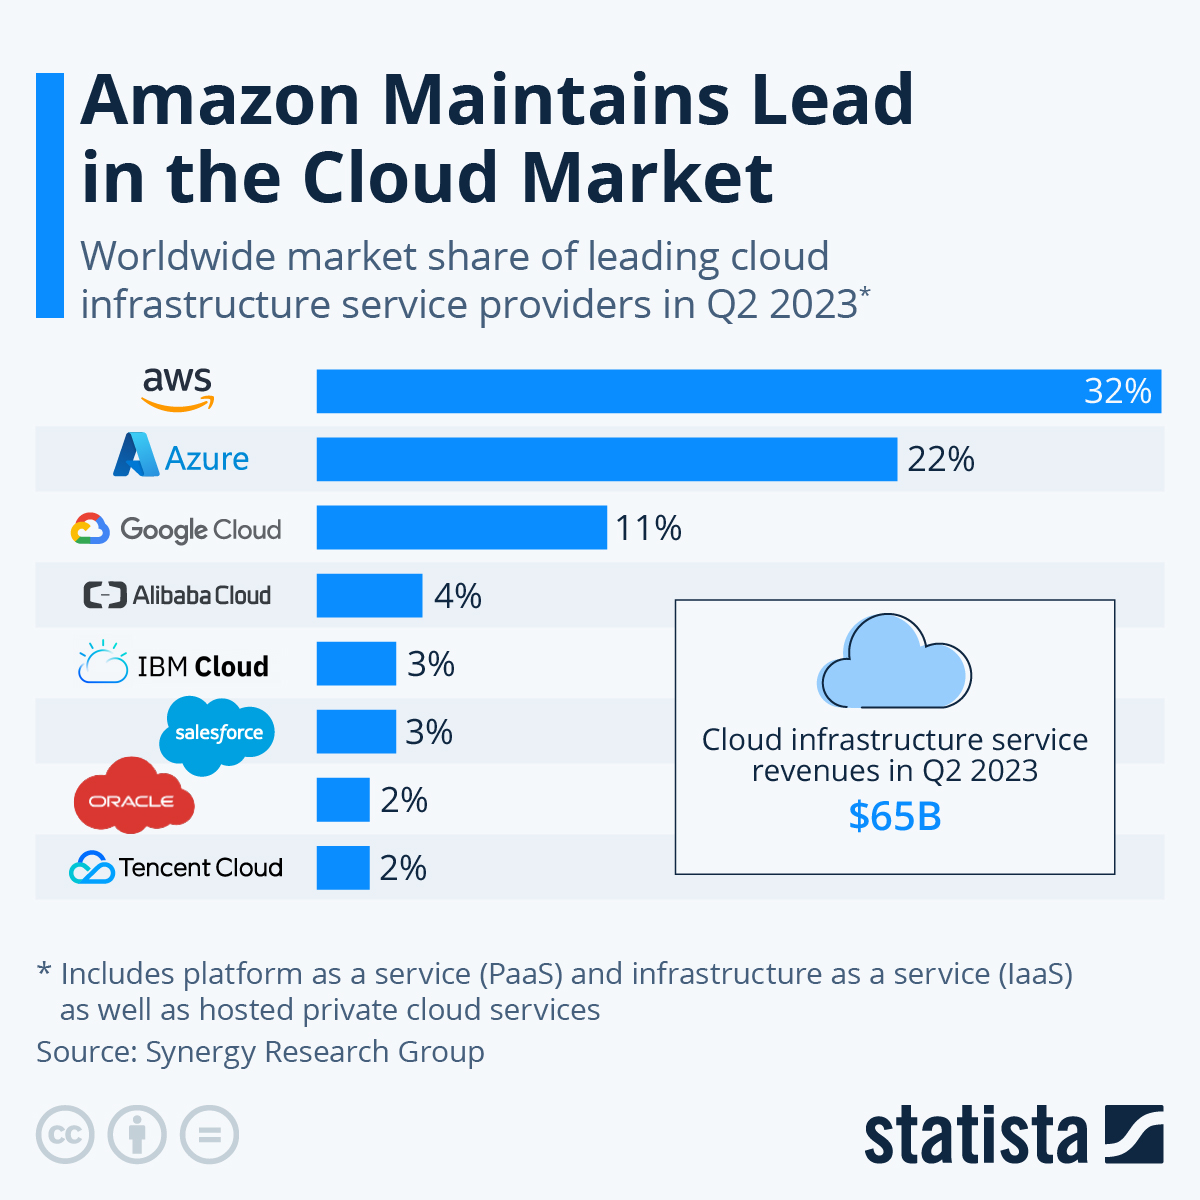
\includegraphics[frame,width=0.7\linewidth]{img/aws/stats.jpeg}
	\captionof{figure}{Fuente: \href{https://www.statista.com/chart/18819/worldwide-market-share-of-leading-cloud-infrastructure-service-providers/}{Statista}}
\end{center}


Entre los proveedores más conocidos de nube pública están:

\begin{itemize}
	\item \textbf{\href{https://aws.amazon.com/es/}{Amazon Web Services}} (AWS): Aunque el negocio inicial de Amazon era el de la venta de libros \textit{online}, durante la creación de un negocio para la creación de tiendas online a terceros se dieron cuenta que sus sistemas internos no tenían la velocidad adecuada.
	
	Decidieron reimplementar toda la infraestructura utilizando estándares abiertos y el sistema \href{https://en.wikipedia.org/wiki/REST}{REST} para la comunicación. En el 2002 lanzó los primeros servicios pero el auge fue en el 2006 cuando lanzó \textbf{EC2} para la generación de máquinas virtuales.
	
	\item \textbf{\href{https://azure.microsoft.com/es-es/}{Microsoft Azure}}: Es la segunda empresa de nube pública. Aunque es la plataforma de Microsoft, Linux es el sistema más utilizado dentro de la virtualización de servicios.
	
	\item \textbf{\href{https://cloud.google.com/}{Google Cloud Platform}}: Google no se podía quedar atrás y también ofrece su sistema de nube pública. Ofrece muchos servicios y zonas de computación, y con la creación del sistema de orquestación de contenedores Kubernetes en 2015, consiguió buena cuota de mercado.
	
	\item \textbf{\href{https://www.ibm.com/cloud}{IBM / Softlayer}}: El sistema de nube público actual de IBM fue inicialmente conocido como SoftLayer, ya que posteriormente lo compró IBM. Aunque se inició en 2005, hoy en día su cuota de mercado no es muy alta.
	
	\item \textbf{\href{https://www.alibabacloud.com/}{Alibaba Cloud}}: Aunque en occidente es posible que no lo conozcamos, Alibaba es un gigante tecnológico en Asia que está detrás de AliExpress, entre otros servicios.  Su cuota de mercado es baja a nivel global, pero muy alta en Asia.
	
\end{itemize}
